% begin legal preamble -- {{{
%%%%%%%%%%%%%%%%%%%%%%%%%%%%%%%%%%%%%%%%%%%%%%%%%%%%%%%%%%%%%%%%%%%%%%%%%%%%%%%%%
% Waterloo Rocketry Standard template for operations procedures                 %
% Copyright claimed by Aaron Morrison (akmorris@uwaterloo.ca)                   %
% Any commercial entity wishing to use this template in any way must provide    %
% to Waterloo Rocketry, one two-four (24 pack) of a non-shitty                  %
% type of beer or an amount of Canadian dollars roughly equalling               %
% the current cost of such a purchase. If you do so, then use it                %
% however you want, and I claim in no way that it compiles properly,            %
% and I take no responsibilty for any loss you incurr from using                %
% this template, and make no promises to support you in any technical           %
% capacity for sustained use.                                                   %
%%%%%%%%%%%%%%%%%%%%%%%%%%%%%%%%%%%%%%%%%%%%%%%%%%%%%%%%%%%%%%%%%%%%%%%%%%%%%%%%%
% end legal preamble -- }}}

\documentclass[letter]{article}

% begin package declarations -- {{{
\usepackage[margin=1in]{geometry}
\usepackage{amsmath}
\usepackage{graphicx}
\usepackage[dvipsnames]{xcolor}
\usepackage{tabto}
\usepackage{titling}
\usepackage[iso,german]{isodate}
\usepackage{titlesec}
\usepackage{float}
\usepackage{caption}
\usepackage{url}
% begin package declarations -- }}}

% begin tikz stuff -- {{{
% tikz gets its own section because its awful
\usepackage{tikz}
\usetikzlibrary{shapes,arrows}
\tikzset{%
  block/.style    = {draw, thick, rectangle, minimum height = 3em,
    minimum width = 3em},
  sum/.style      = {draw, circle, node distance = 2cm}, % Adder
  input/.style    = {coordinate}, % Input
  output/.style   = {coordinate} % Output
}
% end tikz stuff -- }}}

% begin checklist symbols definition -- {{{
\usepackage{enumitem,amssymb}
\newcounter{checklistnum}
\setcounter{checklistnum}{0}
\DeclareRobustCommand{\checklistnumber}{\refstepcounter{checklistnum}\thechecklistnum}
\newlist{checklist}{itemize}{6}
\setlist[checklist,1]{
label={\color{gray}\checklistnumber}\hspace{2em}$\square$,
leftmargin=0em,
itemindent=2em
}
\setlist[checklist,2]{
label={\color{gray}\checklistnumber}\hspace{4em}$\square$,
leftmargin=0em,
itemindent=4em
}
\setlist[checklist,3]{
label={\color{gray}\checklistnumber}\hspace{6em}$\square$,
leftmargin=0em,
itemindent=6em
}
\setlist[checklist,4]{
label={\color{gray}\checklistnumber}\hspace{8em}$\square$,
leftmargin=0em,
itemindent=8em
}
\setlist[checklist,5]{
label={\color{gray}\checklistnumber}\hspace{10em}$\square$,
leftmargin=0em,
itemindent=10em
}
\setlist[checklist,6]{
label={\color{gray}\checklistnumber}\hspace{12em}$\square$,
leftmargin=0em,
itemindent=12em
}
% end checklist symbols definition -- }}}

\titleformat{\section} {\normalfont\Large\bfseries}{}{0em}{}[{\titlerule[0.8pt]}]
\titleformat{\subsection} {\normalfont\large}{}{0em}{}[{\titlerule[0.6pt]}]
\titleformat{\subsubsection} {\bfseries}{}{0em}{}[]

\begin{document}
% begin titlepage -- {{{
\pagenumbering{gobble}
\begin{center}
\vspace*{7cm}
\hspace{7em}
\includegraphics[width=30em]{images/mono_horizontal_standard}
\newline
\rule{50em}{2pt}

\vspace{1cm}
\Huge Remote Launch Control System

\vspace*{\fill}
\small Compiled on \today
\end{center}
\newpage
\pagenumbering{arabic}
% end titlepage -- }}}

% begin Purpose -- {{{
\section{Description of Purpose}
Waterloo Rocketry's Remote Launch Control System (RLCS) is the system that
controls all propellant loading and other preflight actuations required to
launch our rocket.
% end Purpose -- }}}

% begin Design Constraints -- {{{
\section{Design Constraints}
% end Design Constraints -- }}}

% begin Diagrams -- {{{
\section{Block Diagrams}
\begin{figure}[H]
\centering
\scalebox{.8}{
% begin first diagram -- {{{
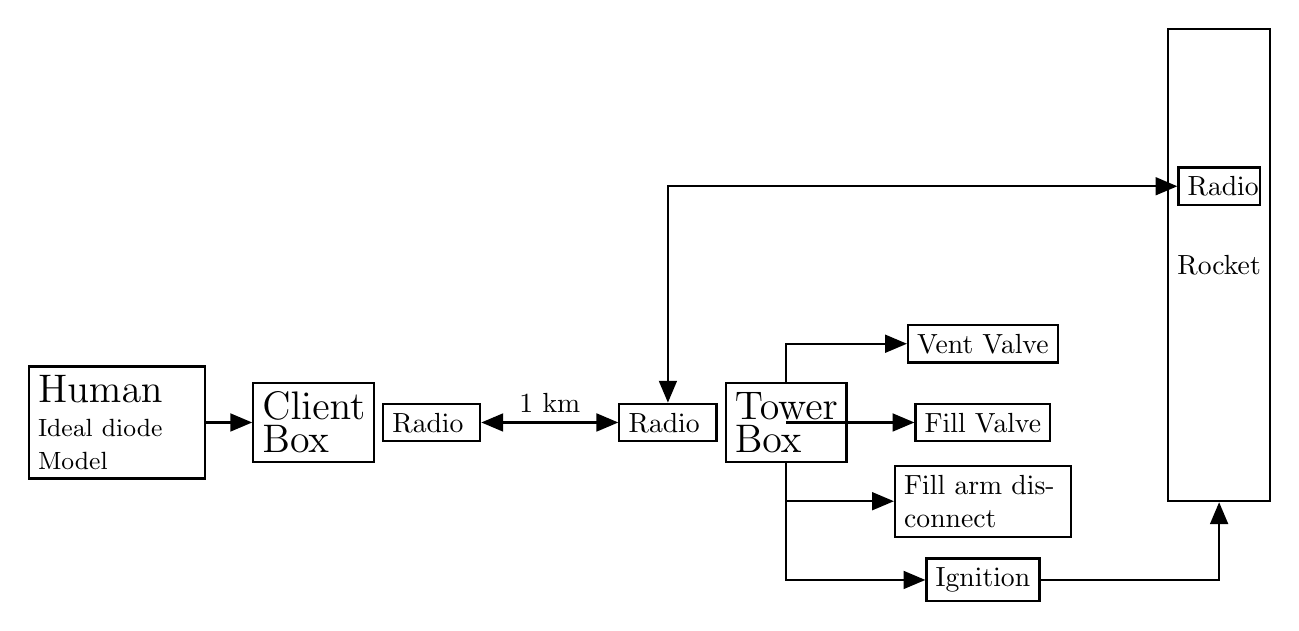
\begin{tikzpicture}[auto, thick, node distance=2cm, >=triangle 45]

%\draw [color=black,thick](-1.5,-1.5) rectangle (1,1);
\draw
    node at(0,0)[text width=2cm,draw,name=miranda]{\Large Human {\small Ideal diode Model}}

    node at(2.5,0)[text width=1.3cm,draw,name=csrf]{\Large Client Box}

    node at(4,0)[text width=1cm,draw,name=crad]{Radio}

    node at(7,0)[text width=1cm,draw,name=trad]{Radio}
    node at(8.5,0)[text width=1.3cm,draw,rectangle,name=tsrf]{\Large Tower Box}

    node at(11,0)[draw,name=RFV]{Fill Valve}
    node at(11,1)[draw,name=RVV]{Vent Valve}
    node at(11,-1)[draw,text width=2cm,name=DCN]{Fill arm disconnect}
    node at(11,-2)[draw,name=IGN]{Ignition}

    node at(14,3)[text width=0.8cm,draw,name=rrad]{Radio}
    node at(14,2)[minimum height=6cm,draw,name=kismet]{Rocket}
;
	\draw[->](miranda) -- (csrf);

    \draw[<->](crad) -- node{1 km}(trad);
    \draw[<->](trad) |- node{}(rrad);

    \draw[->](tsrf) |- (RVV);
    \draw[->](tsrf) |- (RFV);
    \draw[->](tsrf) |- (DCN);
    \draw[->](tsrf) |- (IGN);

    \draw[->](IGN) -| (kismet);

\end{tikzpicture}
% end first diagram -- }}}
}
\caption{High-level System Overview}
\end{figure}

RLCS is composed of two parts, the client side box and the tower side box.
The client side box interfaces with the operator through a bunch of switches
and a big LCD that displays sensor data. The tower side box controls all of
the actuators necessary to launch the rocket (2 valves, nichrome coils, and 
the disconnect linear actuator). In addition to controlling the actuators, the
tower box communicates with two other components in the rocket in order to 
control the two ball valves mounted in the rocket (see documentation of the
flight instrumentation system for more details).

The client box and tower box communicate over a pair of XBEE Pro S3B
transceivers both using half dipole antennas with a gain of 3dBi each. The
tower box communicates with flight instrumentation using XBEE series 1
transceivers all of which have a small whip antenna. The XBEE Pro's operate
at 900MHz, while the series 1's communicate at 2.4GHz.

\begin{figure}[H]
\centering
\scalebox{.8}{
% begin second diagram -- {{{
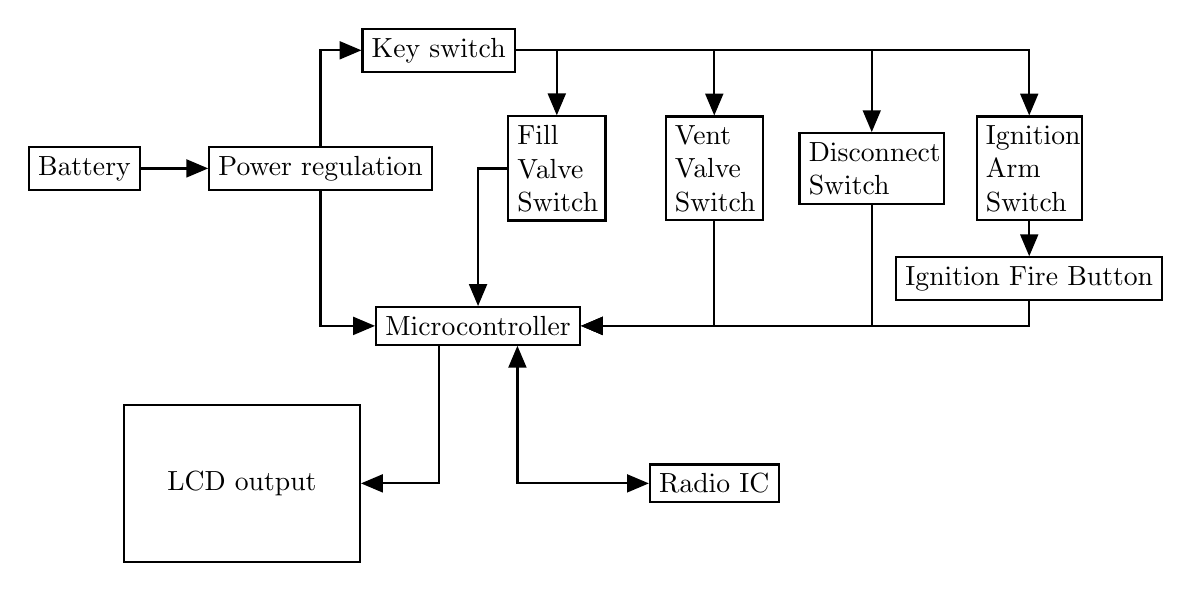
\begin{tikzpicture}[auto, draw, thick, node distance=2cm, >=triangle 45]
\draw
    node at(-3,0)[draw,name=batt]{Battery}
    node at(0,0)[draw,name=reg]{Power regulation}
    node at(1.5,1.5)[draw,name=keysw]{Key switch}

    node at(3,0)[text width=1cm,draw,name=fillsw]{Fill Valve Switch}
    node at(5,0)[text width=1cm,draw,name=ventsw]{Vent Valve Switch}
    node at(7,0)[text width=1.6cm,draw,name=discsw]{Disconnect Switch}
    node at(9,0)[text width=1.1cm,draw,name=igarsw]{Ignition Arm Switch}
    node at(9,-1.4)[draw,name=igfisw]{Ignition Fire Button}

    node at(2,-2)[draw,name=ard]{Microcontroller}

    node at (-1,-4)[minimum height=2cm,minimum width=3cm,draw,name=lcd]{LCD output}

    node at (5,-4)[draw,name=crad]{Radio IC}
;

    \draw[->](batt) -- (reg);
    \draw[->](reg) |- (keysw);
    \draw[->](keysw) -| (fillsw);
    \draw[->](keysw) -| (ventsw);
    \draw[->](keysw) -| (discsw);
    \draw[->](keysw) -| (igarsw);
    \draw[->](igarsw) -- (igfisw);

    \draw[->](reg) |- (ard);

    \draw[->](fillsw) -| (ard);
    \draw[->](ventsw) |- (ard);
    \draw[->](discsw) |- (ard);
    \draw[->](igfisw) |- (ard);

    \draw[->](ard.south) + (-0.5,0) |- (lcd);
    \draw[<->](ard.south) + (0.5,0) |- (crad);
\end{tikzpicture}
% end second diagram -- }}}
}
\caption{Client side block-level diagram}
\end{figure}

The client side box is composed of a number of switches connected to a 
microcontroller (in this case, an Arduino Mega), which is in turn connected
to an LCD (to relay information to the user) and the radio transceiver. All
switches are connected in series with a keyswitch to allow the system to be
disabled whenever personnel are nearby the rocket. The ignition switch is in
series with a momentary pushbutton to remove the possibility of a switch being
left in the the "fire" position when the system is first started. The "power
regulation" board is a switching regulator which drops the 11.1v from the battery
to 5v, which can be used by the microcontroller.

\begin{figure}[H]
\centering
\scalebox{.8}{
% begin third diagram -- {{{
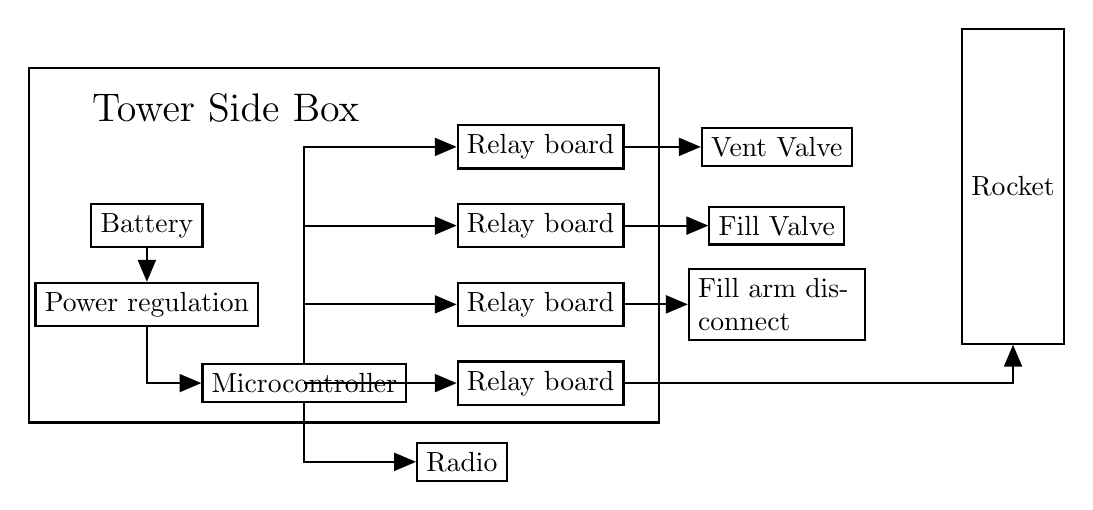
\begin{tikzpicture}[auto,draw,thick,node distance=2cm, >=triangle 45]
\draw
    node at(0,0)[draw,name=batt]{Battery}
    node at(0,-1)[draw,name=reg]{Power regulation}
    node at(2,-2)[draw,name=ard]{Microcontroller}

    node at (5,1)[draw,name=cb1]{Relay board}
    node at (5,0)[draw,name=cb2]{Relay board}
    node at (5,-1)[draw,name=cb3]{Relay board}
    node at (5,-2)[draw,name=cb4]{Relay board}
    node at (4,-3)[draw,name=rad]{Radio}

    node at (8,1)[draw,name=rvv]{Vent Valve}
    node at (8,0)[draw,name=rfv]{Fill Valve}
    node at (8,-1)[draw,name=dis,text width=2cm]{Fill arm disconnect}
    node at (11,0.5)[minimum height=4cm,draw,name=kismet]{Rocket}
    node at (1,1.5)[]{\Large Tower Side Box}
;

    \draw [color=black,thick](-1.5,-2.5) rectangle (6.5,2);
    \draw[->](batt) -- (reg);
    \draw[->](reg) |- (ard);
    \draw[->](ard) |- (rad);
    \draw[->](ard) |- (cb1);
    \draw[->](ard) |- (cb2);
    \draw[->](ard) |- (cb3);
    \draw[->](ard) |- (cb4);

    \draw[->](cb1) -- (rvv);
    \draw[->](cb2) -- (rfv);
    \draw[->](cb3) -- (dis);
    \draw[->](cb4) -| (kismet);

	%\draw [color=gray,thick](-0.5,-9) rectangle (12.5,-5);
\end{tikzpicture}
% end third diagram -- }}}
}
\caption{Tower side block-level diagram}
\end{figure}

The tower side box controls external actuators through relay boards, which are
cutomed designed PCBs that feature a DPDT relay, for changing direction of valves
or swapping between ignition circuits, and an SPST relay, for interrupting current
to the actuator when it is set to off. The boards also feature current sensors on
all actuator outputs, and logic level shifting for the limit switch signals coming
off of the valve, dropping the signal from 12 volts to 5, which the microcontroller
can read. The batteries in this box (as well as all other batteries the system uses)
are fused to prevent a fire in the event of power ever being shorted to ground.
% end Diagrams -- }}}

% begin Functionality -- {{{
%\section{Functionality}

%This system works by a bunch of black magic fuckery.
% end Functionality -- }}}

% begin Tradeoffs -- {{{
\section{Tradeoffs}
% end Tradeoffs -- }}}

% begin Analysis -- {{{
\section{Analysis/testing}
Here's why this doesn't break a bunch of rules.

\subsection{Design, Test, \& Evaluation Guide}
\subsubsection{Rule 2.2 - PROPULSION SYSTEM SAFING AND ARMING}
\begin{itemize}
\item {\bfseries ``A propulsion system is considered armed if only one action 
(eg an ignition signal) must occur for the propellant(s) to ignite''}

Our propellant is really hard to ignite. We've performed numerous tests to determine
if our fuel grain (main propellant) can be ignited without nitrous oxide present.
We've never managed to ignite it. Using that as precedent, we can say
that our ignition system isn't armed until oxidizer is present in our flight tank.
Since oxidizer alone isn't enough to ignite our propellant without extreme heat also
present, you could make the argument that our ignition system isn't really armed until
the ignition puck is burning \textit{and} there is oxidizer present in our flight tank.
\end{itemize}
\subsubsection{Rule 2.2.1 - GROUND-START IGNITION CIRCUIT ARMING}
\begin{itemize}
\item {\bfseries ``All ground-started propulsion system ignition circuits/sequences shall not be ``armed'' until all personnel are at least
50 ft (15 m) away from the launch vehicle.''}

Our operations procedures ensure that there is never oxidizer in our flight tank
until we are ready to launch, and all personnel are already at the minimum safe
distance away from the rocket. We do not arm our ignition sequences until all
personnel are much further than 15m away from the vehicle.
\end{itemize}
\subsubsection{Rule 2.2.3 - PROPELLANT OFFLOADING AFTER LAUNCH ABORT}
\begin{itemize}
\item {\bfseries ``Hybrid and liquid propulsion systems shall implement a means for remotely controlled venting or offloading of all
liquid and gaseous propellants in the event of a launch abort''}

We have a 0.3mm diameter hole in series with an electrically controlled valve in our
rocket to facilitate offloading of all liquid propellant in the event of an abort.
Before going to the competition, we perform a full systems integration test in which
we fill the rocket with CO$_2$ and then vent all of it to ensure that this system is
operational and functions properly. TODO Jacob do we still do this?
\end{itemize}
\subsubsection{Rule 3.4 - SAFETY CRITICAL WIRING}
\begin{itemize}
\item {\bfseries ``Safety critical wiring is defined as electrical wiring associated with recovery system
deployment events and any ``air started'' rocket motors''}

This system is in no way associated with either of those things, which is why
it does not (in some minor places) comply with the safety critical wiring
standard.
\end{itemize}
\subsubsection{Rule 4.1 - ENERGETIC DEVICE SAFING AND ARMING}
\begin{itemize}
\item {\bfseries ``All energetics shall be safed until the rocket is in the launch position, at which point they may be ``armed''. An energetic
device is considered safed when two separate events are necessary to release the energy''}

Our ignition system contains two nichrome igniters embedded in a flammable solid
fuel puck, which is the only energetic associated with this system. Until the
rocket is mounted on the rail, these igniters are shorted and are not connected
to the system, and thus they are not armed, since you'd have to un-short them and
then plug them in before the energy can be released.
\end{itemize}
\subsubsection{10.1 EQUIPMENT PORTABILITY}
\begin{itemize}
\item {\bfseries ``Teams should make their launch support equipment man-portable over a short distance (a few
hundred feet)''}

The tower side box component of this system is the heaviest piece, which weighs
12lbs and has a handle on it for ease of portability. The entire system is
easily man portable and can be carried by 2 or 3 people well over a few hundred
feet.
\end{itemize}
\subsubsection{10.3 OPERATIONAL RANGE}
\begin{itemize}
\item {\bfseries ``All team provided launch control systems shall be electronically operated and have a maximum operational range of
no less than 2,000 ft (~610 m) from the launch rail''}

Our system is electronically operated and uses two XBEE-PRO XSC S3B modules
which have an advertised range of 28 miles with line of sight. We used the
exact same modules last year and had no issues with loss of communication.
\end{itemize}
\subsubsection{10.4 FAULT TOLLERANCE AND ARMING}
\begin{itemize}
\item {\bfseries ``All team provided launch control systems shall be at least single fault tolerant by implementing a removable safety
interlock (i.e. a jumper or key to be kept in possession of the arming crew during arming) in series with the launch
switch''}

We use a key switch in series with all other control switches on our client
side box. The key is held by either an IREC official or the arming crew until
the rocket is ready to launch.
\end{itemize}
\subsubsection{10.5 SAFETY CRITICAL SWITCHES}
\begin{itemize}
\item {\bfseries ``All team provided launch control systems shall implement ignition switches of the momentary, normally open (aka
``deadman'') type''}

Our ignition actuation button is momentary and normally open.
\end{itemize}
\subsubsection{APPENDIX C: FIRE CONTROL SYSTEM DESIGN GUIDLINES}
\begin{itemize}
\item {\bfseries ``The control console should be designed such that two deliberate actions are
required to fire the system''}

Since all switches are in series with the keyswitch, any action taken at the
control box really takes 4 deliberate actions (put key in box, turn key,
flip up switch cover, actuate switch). Because the ignition fire button is
in series with two missile switches, firing the system takes 5 deliberate
actions, and 5 is greater than two for all values of 5 (insert key, turn key,
flip up switch cover, actuate switch, press button).

\item {\bfseries ``The system should include a power interrupt such that firing current cannot be
sent to the firing leads while personnel are at the pad and this interrupt
should be under the control of personnel at the pad.''}

Does the keyswitch count?

\item {\bfseries ``The failure of any single component should not compromise the safety of the
firing system.''}

Our ignition system requires at minimum 3 separate actions to occur (open fill valve, send 
ignition current, open injector valve) before our ignition system actuates. There is no
single component that can fail that would cause all three of these actions to occur (unless
a microcontroller fails in an impossibly specific and malicious way), and thus our the
safety of our system would never be compromised by a single component's failure. All subsystems
are designed to fail safe (certain valves close in the event of communications loss, there
are inline fuses on all actuator power lines, etc) in the event of component failure.
\end{itemize}
% end Analysis -- }}}

% begin Shameless self promotion -- {{{
\section{Glamour shots}

\begin{figure}[H]

\centering
\begin{minipage}{.36\textwidth}
  \centering
  \includegraphics[width=.9\linewidth]{images/clientside}
  \captionof{figure}{The clientside box}
  \label{fig:test1}
\end{minipage}%
\begin{minipage}{.64\textwidth}
  \centering
  \includegraphics[width=.9\linewidth]{images/towerside}
  \captionof{figure}{The towerside box}
  \label{fig:test2}
\end{minipage}

\end{figure}

% end Shameless self promotion -- }}}

% begin Nerd stuff -- {{{
\section{Technical Details and Schematics if you're \textit{really} interested}

All technical specifications (from schematics and layouts down to individual
component datasheets) can be found in this project's github repository,
\url{https://github.com/waterloo-rocketry/rlcs}. Also present in that repository
is all the code that runs on the microcontrollers, all the unit tests that that
code is checked against, and also this document.
% end Nerd stuff -- }}}

% begin Checklists -- {{{
\section{Assembly and Pre-Launch Checklists}
The order of operations:
\begin{checklist}
    \item When RLCS takes over, here's the current state of our fill system: 
    \begin{checklist}
        \item The NOs K bottle's cylinder valve is open 
        \item The plumbing system is set up, all valves are closed (except series
              fill)
        \item The only pressurized line is the fill line (leads from cylinder to
              remote fill valve). All other lines are atmospheric.
    \end{checklist}
    \item The primary operator marks the current fill line pressure (reads from SP1)
    \item The primary operator opens the rocket vent valve, which will allow the
            rocket to be fuelled.
    \item The primary operator opens the remote fill valve, pressurizing the feed
            line.  Oxidizer begins to flow into the run tank, while fumes vent from the
            top of the run tank through the rocket vent valve. At this moment (oxidizer in
            the run tank), our ignition system and rocket are considered armed. All
            personnel must be at the Minimum safe distance before this point.
    \item Once the rocket is fuelled (as indicated be the primary load cell and rocket
            pressure transducer), the rocket vent valve is closed, sealing the run tank.
    \item The remote fill valve is closed, sealing the supply tank off from the rest
            of the plumbing assembly.  
    \item The remote vent valve is opened, venting the feed line, so that is at
            atmospheric pressure. The goal of this step is to allow the remote
            disconnect arm to swing free without spraying the airframe of the rocket
            with oxidizer.
    \item The remote disconnect pin is pulled, allowing the fill arm to swing free.
            The rocket is now disconnected from the fill system, and ready to launch.
            because of the one way check valve in the rocket, the nitrous does not vent
            through the fill arm adapter)
    \item Once the IREC official says so, we can actuate ignition and launch:
    \begin{checklist}
        \item Ignition is fired, igniting the puck in the CC.
        \item Once we have confirmation of flame in the CC (read from ammeter on
                ignition circuit), we open the injector valve.
        \item Watch the rocket, because this'll be pretty cool.
    \end{checklist}
\end{checklist}

End of Operations.
% end Checklists -- }}}

\end{document}
